\documentclass[11pt]{article}
\usepackage[margin=1in]{geometry}
\usepackage{amsmath,amssymb,amsthm}
\usepackage{physics}
\usepackage{hyperref}
\usepackage{cancel}
\usepackage{pgfplots}
\pgfplotsset{compat=1.18}
\usepgfplotslibrary{fillbetween}

\newtheorem*{problem}{Problem}
\newtheorem*{solution}{Solution}

\begin{document}

\noindent
\begin{minipage}[t]{0.5\textwidth}
\raggedright
\Large Statistical Physics examples solutions 1
\end{minipage}%
\begin{minipage}[t]{0.5\textwidth}
\raggedleft
Billy Adamson
\end{minipage}

\vspace{1em}

\begin{problem}
1. Establish Stirling's formula as follows. Start with
\[
n! = \int_0^\infty e^{-x}x^n\,dx \equiv \int_0^\infty e^{-F(x)}\,dx.
\]
Let the minimum of $F$ be at $x_0$. Approximate $F(x)$ by $F(x_0)+F''(x_0)(x-x_0)^2/2$.
(One further approximation is needed.) Hence obtain $n! \sim \sqrt{2\pi n}\,n^n e^{-n}$, and the
statistical physics approximation $\ln n! \sim n\ln n - n$.
\end{problem}

\begin{solution}
\[
n! = \int_0^\infty e^{-x}x^n\,dx
= \int_0^\infty e^{-F(x)}\,dx,
\qquad
F(x)=x-n\ln x.
\]

\[
F'(x_0)=1-\frac{n}{x_0}=0
\quad\Rightarrow\quad
x_0=n.
\]

\[
F''(x)=\frac{n}{x^2}
\quad\Rightarrow\quad
F''(n)=\frac{1}{n}.
\]

\[
F(x)\approx F(n)+\frac{1}{2}F''(n)(x-n)^2
=
\left(n-n\ln n\right)
+\frac{(x-n)^2}{2n}.
\]

\[
n!\approx
\int_0^\infty
\exp\!\left[
-F(n)
-\frac{(x-n)^2}{2n}
\right]
dx
=
e^{-F(n)}
\int_0^\infty
\exp\!\left[
-\frac{(x-n)^2}{2n}
\right]
dx.
\]

This is a Gaussian in $x$, centred at $x_0=n$ with standard deviation $\sqrt{n}$.
The lower limit $x=0$ is $\sqrt{n}$ below the peak (i.e.\ $\sqrt{n}$ standard deviations away),
so the region $x<0$ contributes negligibly; it is therefore reasonable
to extend the lower limit to $-\infty$:

\begin{center}
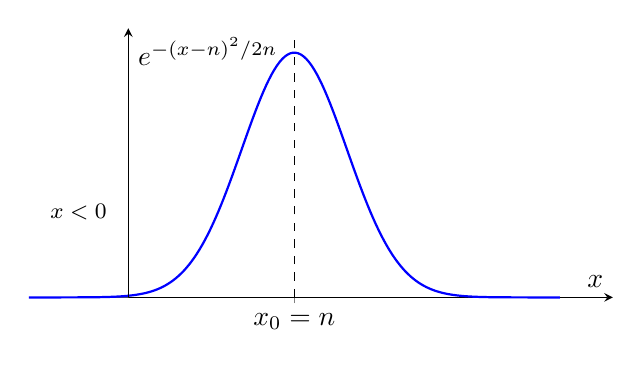
\begin{tikzpicture}
\begin{axis}[
  width=9cm, height=5cm,
  domain=-6:26,
  samples=200,
  axis lines=middle,
  xlabel={$x$}, ylabel={$e^{-(x-n)^2/2n}$},
  xtick={0,10}, xticklabels={$0$,$x_0=n$},
  ytick=\empty,
  clip=false,
  enlargelimits=upper,
]
\addplot [name path=gauss, thick, blue, domain=-6:26] {exp(-(x-10)^2/20)};
\addplot [name path=axis, draw=none] {0};
\addplot [blue!15] fill between [of=gauss and axis, soft clip={domain=-6:0}];
\draw [dashed] (axis cs:0,0) -- (axis cs:0,1.05);
\draw [dashed] (axis cs:10,0) -- (axis cs:10,1.05);
\node at (axis cs:-3,0.35) {\footnotesize $x<0$};
\end{axis}
\end{tikzpicture}
\end{center}

Using the standard Gaussian integral $\displaystyle\int_{-\infty}^{\infty} e^{-(x-a)^2/2\sigma^2}\,dx=\sqrt{2\pi\sigma^2}$,

\[
n!\approx
e^{-F(n)}
\int_{-\infty}^{\infty}
\exp\!\left[
-\frac{(x-n)^2}{2n}
\right]
dx
=
e^{-F(n)}\sqrt{2\pi n}.
\]

\[
n! \approx e^{-F(n)}\sqrt{2\pi n} = e^{-n+n\ln n}\sqrt{2\pi n}.
\]

\[
\boxed{n! \sim \sqrt{2\pi n}\, n^n e^{-n}}
\]

\[
\boxed{\ln n! \sim n\ln n - n}
\]
\end{solution}

\begin{problem}
2. A cubic box is described by a three-dimensional infinite square well with $0\le x,y,z\le a$
and corresponding single-particle energy eigenstates
\[
E=\frac{\hbar^2\pi^2}{2ma^2}(p^2+q^2+r^2)
\]
where $p,q,r$ are positive integers. Assume that the box contains $N$ non-interacting
distinguishable particles of mass $m$. Let $G(E)$ be the number of states with energy less
than $E$. For $E \gg \hbar^2\pi^2/(2ma^2)$ show that $G(E) \approx cE^{\alpha N}$ for some
positive constants $c$ and $\alpha$. Determine the value of $\alpha$.

[\textit{Hint}: a microstate can be parameterized by $3N$ positive integers and states with
energy less than $E$ are those for which these integers lie inside some sphere in the
corresponding $3N$ dimensional space. How does the volume of this sphere depend on $N$?]
\end{problem}

\begin{solution}
\[
E=\frac{\hbar^2\pi^2}{2ma^2}(p^2+q^2+r^2),
\qquad p,q,r\in\mathbb{Z}^+.
\]

\[
E=\frac{\hbar^2\pi^2}{2ma^2}\sum_{i=1}^{N}(p_i^2+q_i^2+r_i^2).
\]

\[
\sum_{i=1}^{N}(p_i^2+q_i^2+r_i^2)
<
\frac{2ma^2E}{\hbar^2\pi^2}.
\]

The allowed microstates are discrete coordinate points inside a $3N$-dimensional sphere
of radius

\[
R=\left(\frac{2ma^2E}{\hbar^2\pi^2}\right)^{1/2}.
\]

Since $E$ is large, the points are densely packed and counting them is well approximated
by the volume of the sphere,

\[
V_{3N}
=
\frac{\pi^{3N/2}}
{\Gamma\!\left(\frac{3N}{2}+1\right)}
R^{3N}.
\]

\[
G(E)
\approx
\frac{\pi^{3N/2}}
{\Gamma\!\left(\frac{3N}{2}+1\right)}
\left(\frac{2ma^2E}{\hbar^2\pi^2}\right)^{3N/2}.
\]

\[
G(E)\approx c\,E^{\alpha N},
\]

\[
c=
\frac{\pi^{3N/2}}
{\Gamma\!\left(\frac{3N}{2}+1\right)}
\left(\frac{2ma^2}{\hbar^2\pi^2}\right)^{3N/2},
\]

\[
\boxed{\alpha=\frac{3}{2}.}
\]
\end{solution}

\begin{solution}
\subsection*{(i)}

\[
\Omega_i(E)=c_iE^{\alpha_iN_i},
\]

\[
p(E_1)\propto \Omega_1(E_1)\Omega_2(E-E_1)
\propto E_1^{\alpha_1N_1}(E-E_1)^{\alpha_2N_2}.
\]

\[
\ln p(E_1)
=
\text{const}
+\alpha_1N_1\ln E_1
+\alpha_2N_2\ln(E-E_1).
\]

$\ln$ is increasing, so we can differentiate:
\[
\frac{d}{dE_1}\ln p(E_1)
=
\frac{\alpha_1N_1}{E_1}
-
\frac{\alpha_2N_2}{E-E_1}.
\]

\[
\frac{\alpha_1N_1}{E_1^*}
=
\frac{\alpha_2N_2}{E-E_1^*},
\]

\[
\alpha_1N_1(E-E_1^*)
=
\alpha_2N_2E_1^*.
\]

\[
E_1^*
=
\frac{\alpha_1N_1}
{\alpha_1N_1+\alpha_2N_2}\,E.
\]

\subsection*{(ii)}

\[
\ln p(E_1)
\approx
\ln p(E_1^*)
+
\cancelto{0}{\frac{d}{dE_1}\ln p(E_1)}\Big|_{E_1^*}(E_1-E_1^*)
+
\frac12
\left.
\frac{d^2}{dE_1^2}\ln p(E_1)
\right|_{E_1^*}
(E_1-E_1^*)^2.
\]

\[
\frac{d^2}{dE_1^2}\ln p(E_1)
=
-\frac{\alpha_1N_1}{E_1^2}
-
\frac{\alpha_2N_2}{(E-E_1)^2}.
\]

\[
E_1^*
=
\frac{\alpha_1N_1}{\alpha_1N_1+\alpha_2N_2}E,
\qquad
E-E_1^*
=
\frac{\alpha_2N_2}{\alpha_1N_1+\alpha_2N_2}E,
\]

\[
\left.
\frac{d^2}{dE_1^2}\ln p(E_1)
\right|_{E_1^*}
=
-
\frac{(\alpha_1N_1+\alpha_2N_2)^3}
{\alpha_1\alpha_2N_1N_2\,E^2}.
\]

\[
p(E_1)
\approx
p(E_1^*)
\exp\left[
-
\frac{(\alpha_1N_1+\alpha_2N_2)^3}
{2\alpha_1\alpha_2N_1N_2\,E^2}
(E_1-E_1^*)^2
\right].
\]

This is a Gaussian distribution with variance
\[
\sigma^2
=
\frac{\alpha_1\alpha_2N_1N_2}
{(\alpha_1N_1+\alpha_2N_2)^3}
E^2.
\]

Since \(N_1,N_2\approx N\), we have
\[
\sigma
\sim
\frac{E}{\sqrt{N}}.
\]

\[
\boxed{
p(E_1)\text{ is negligible whenever }
|E_1-E_1^*|
\gg
\frac{E}{\sqrt{N}}.
}
\]
\end{solution}

\begin{problem}
4. (a) Show that two coupled systems in the microcanonical ensemble, each with heat
capacity $C$, maximize their entropy at equal temperature only if $C$ is positive.

(b) In the canonical ensemble, show that the fluctuations in energy,
$(\Delta E)^2 = \langle E^2\rangle - \langle E\rangle^2$, are proportional to the heat capacity.

(c) Show that in the canonical ensemble the Gibbs entropy can be written as
$S = k_B\dfrac{\partial}{\partial T}(T\ln Z)$.
\end{problem}

\begin{solution}
\subsection*{(a)}
\[
S_{\text{total}}(E_1)=S_1(E_1)+S_2(E_{\text{total}}-E_1).
\]
Equilibrium:
\[
0=\frac{dS_{\text{total}}}{dE_1}
=\frac{\partial S_1}{\partial E_1}-\frac{\partial S_2}{\partial E_2}
=\frac1{T_1}-\frac1{T_2},
\]
\[
T_1=T_2.
\]

\[
\frac{d^2S_{\text{total}}}{dE_1^2}
=\frac{\partial^2 S_1}{\partial E_1^2}+\frac{\partial^2 S_2}{\partial E_2^2}.
\]
N.B:
\[
\frac{\partial S}{\partial E}=\frac1T,
\qquad
C=\frac{\partial E}{\partial T},
\]
\[
\frac{\partial^2 S}{\partial E^2}
=\frac{d}{dE}\!\left(\frac1T\right)
=-\frac{1}{T^2C}.
\]
Hence, for two identical systems with heat capacity \(C\),
\[
\frac{d^2S_{\text{total}}}{dE_1^2}=-\frac{2}{T^2C},
\]
which is negative iff \(C>0\).
\[
\boxed{C>0}
\]

\subsection*{(b)}
\[
Z=\sum_n e^{-\beta E_n},\qquad
\langle E\rangle=-\frac{\partial}{\partial\beta}\ln Z.
\]
\[
(\Delta E)^2
=\langle E^2\rangle-\langle E\rangle^2
=\frac{\partial^2}{\partial\beta^2}\ln Z
=-\frac{\partial\langle E\rangle}{\partial\beta}.
\]
N.B: \(\beta=\dfrac{1}{k_BT}\),
\[
(\Delta E)^2
=-\frac{\partial\langle E\rangle}{\partial T}\frac{dT}{d\beta}
=k_BT^2\frac{\partial\langle E\rangle}{\partial T}
=\boxed{k_BT^2C_V}.
\]

\subsection*{(c)}
\[
S=-k_B\sum_n p_n\ln p_n,\qquad
p_n=\frac{e^{-\beta E_n}}{Z}.
\]
\[
\ln p_n=-\beta E_n-\ln Z,
\]
\[
S=-k_B\sum_n p_n(-\beta E_n-\ln Z)
=k_B\beta\langle E\rangle+k_B\ln Z.
\]
\[
\frac{\partial}{\partial T}(T\ln Z)
=\ln Z+T\frac{\partial\ln Z}{\partial T}
=\ln Z+\beta\langle E\rangle,
\]
\[
\boxed{S=k_B\frac{\partial}{\partial T}(T\ln Z)}
\]
\end{solution}

\end{document}
